\subsection{Dynamics block}\label{chapter_DYNAMICS_BLOCK}
The MATLAB Simulink block, that includes the physical model of the quadrocopter, pictured in orange in figure \ref{fig:MATLAB Overview}, is the topic of this chapter.
As this model doesn't fit on one page, it is split up into multiple sections. The picture below shows the whole process, divided into four areas. The following chapters discuss these areas as appropriate. It is not necessary to discuss each block in detail, to be able to develop a controller for this process.
\begin{figure}[H]
	\centering
		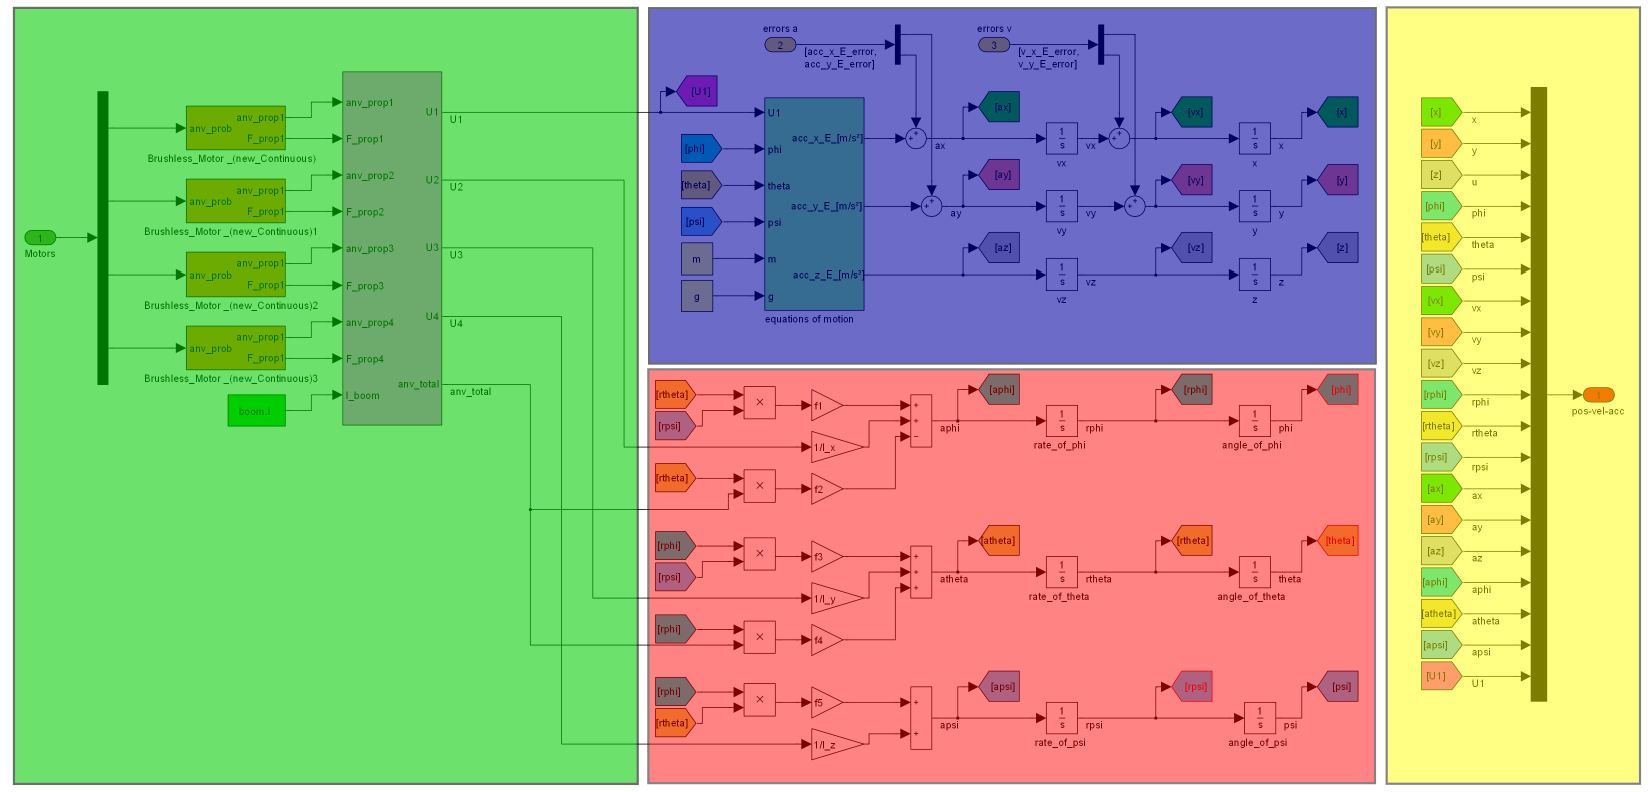
\includegraphics[width=1.0\textwidth]{03_Grafiken/MATLAB_Dynamics_Sections.pdf}
	\caption{Sections of the Dynamics block}
	\label{fig:MATLAB Dynamics Sections}
\end{figure}
\clearpage %neue Seite erzwingen

\subsubsection{Dynamics of the four motors (green section)}\label{chapter_GREEN_SECTION}
The green section has one input vector. It holds the pseudo forces, every propeller has to provide, given by the controller.
\begin{figure}[H]
	\centering
		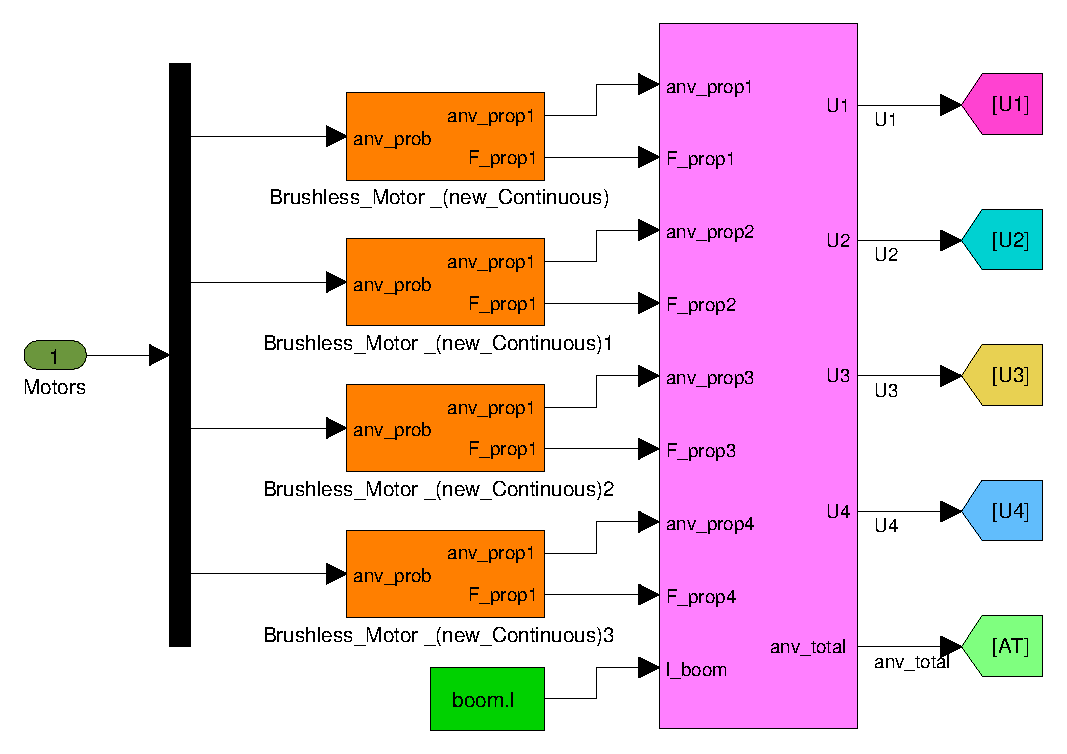
\includegraphics[width=0.8\textwidth]{03_Grafiken/MATLAB_Dynamics1.pdf}
	\caption{Green section}
	\label{fig:MATLAB Dynamics1}
\end{figure}
Each pseudo force is the input of one motor (orange blocks). 
Double clicking on one of the motors opens the graphic below.
\begin{figure}[H]
	\centering
		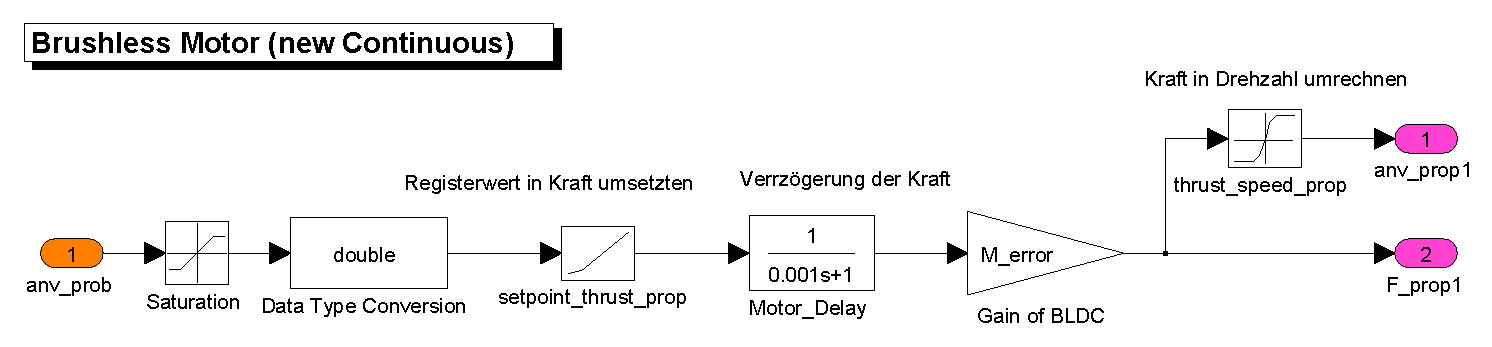
\includegraphics[width=1.0\textwidth]{03_Grafiken/motorWithDelay.pdf}
	\caption{Motor}
	\label{fig:motor}
\end{figure}
The pseudo force, coming from the controller, gets converted into a real force by the characteristic diagram 'setpoint\_thrust\_prop'. Due to the inertia of the propeller this force is delayed by a PT1-element.
The motor has two outputs, \textit{anv\_propX} and \textit{F\_propX}, where \textit{F\_prop} is the force, the propeller produces vertically to itself. \textit{anv\_prop} is the angular velocity of the propeller, that gets calculated by the characteristic diagram 'thrust\_speed\_prop'.

The big purple block in figure \ref {fig:MATLAB Dynamics1} uses these forces to calculate the angular accelerations in direction of phi (U2), theta(U3) and psi(U4). For this calculation the lever principle (force * lever) is used. The small green block \textit{boom.l} provides the information about the levers. 
The purple block also has two other output values \textit{U1} and \textit{AT}. \textit{U1} is the sum of all propeller forces \textit{F\_propX}, \textit{AT} is the sum of all rotary speeds \textit{anv\_propX}.

\subsubsection{Dynamics of quadrocopter in bodyframe (red section)}\label{chapter_RED_SECTION}
This section represents the bodyframe of the quadrocopter and consits of three very similar lines.
\begin{figure}[H]
	\centering
		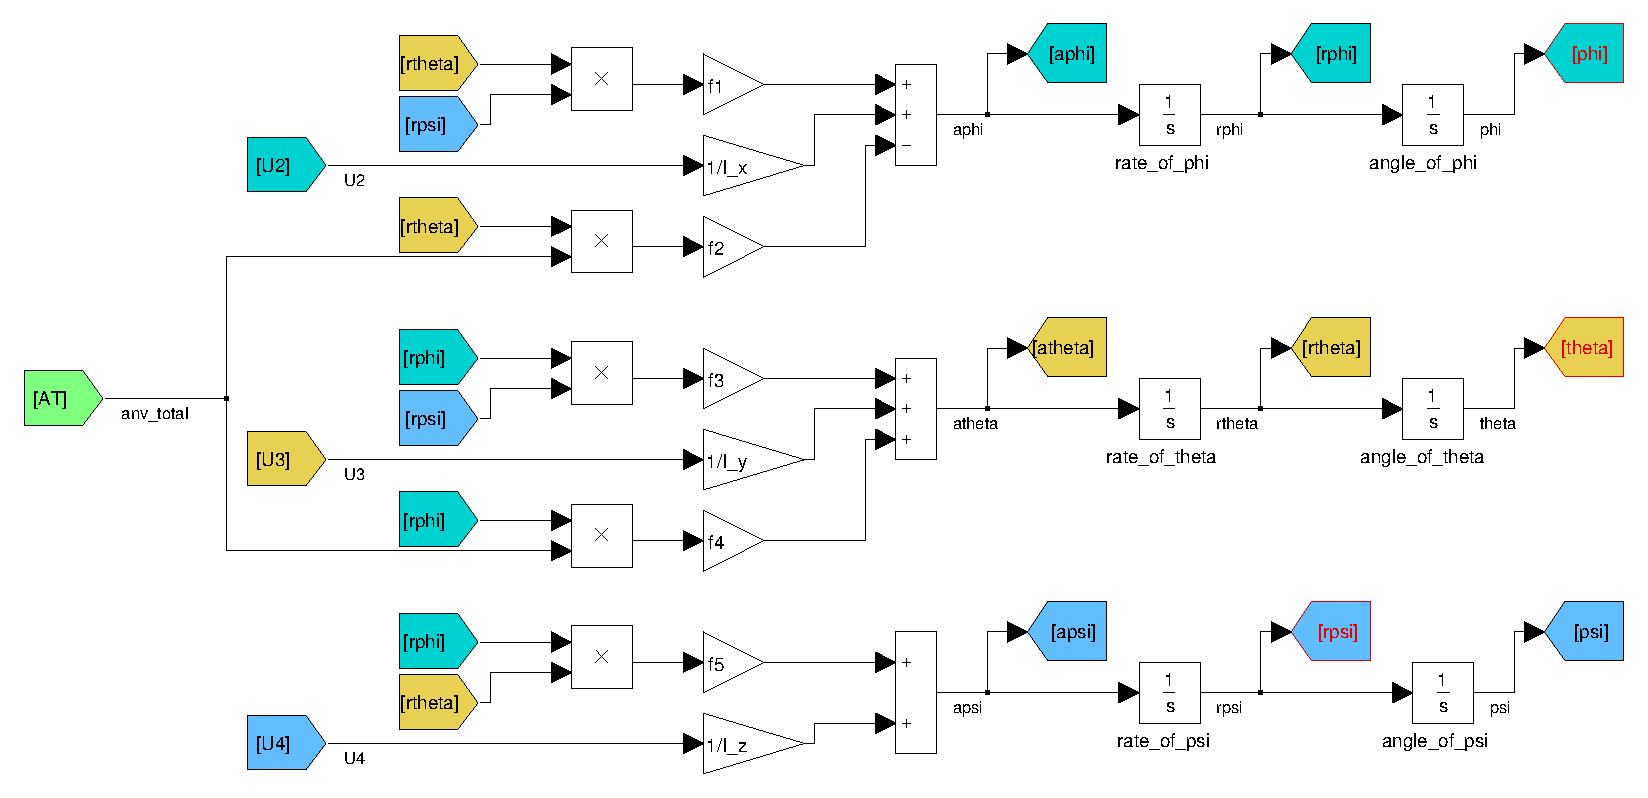
\includegraphics[width=1.0\textwidth]{03_Grafiken/MATLAB_Dynamics2.pdf}
	\caption{Red section}
	\label{fig:MATLAB Dynamics2}
\end{figure}
The topmost line uses the rate of theta \textit{rtheta}, the rate of psi \textit{rpsi}, the angular acceleration in direction of phi \textit{U2} and the sum of all rotary speeds \textit{AT} to calculate the resulting angular acceleration in direction of phi (\textit{aphi}) of the physical model. This shows, that movement in direction of \textit{phi} is influenced by movement in direction of \textit{theta} and \textit{psi}. This is momentous for the development of the controller.\\
The angular acceleration gets integrated once, resulting in the angular rate of phi \textit{rphi}, and twice, resulting in the angle \textit{phi}. The other two lines for \textit{theta} and \textit{psi} are very similar, so this is not discussed here in detail. The controlled variables \textit{phi}, \textit{theta} and \textit{rpsi} are pictured in red letters.
 
\subsubsection{Dynamics of quadrocopter in earthframe (blue section)}\label{chapter_BLUE_SECTION}
While the red section represents the bodyframe, this section represents the earthframe.
\begin{figure}[H]
	\centering
		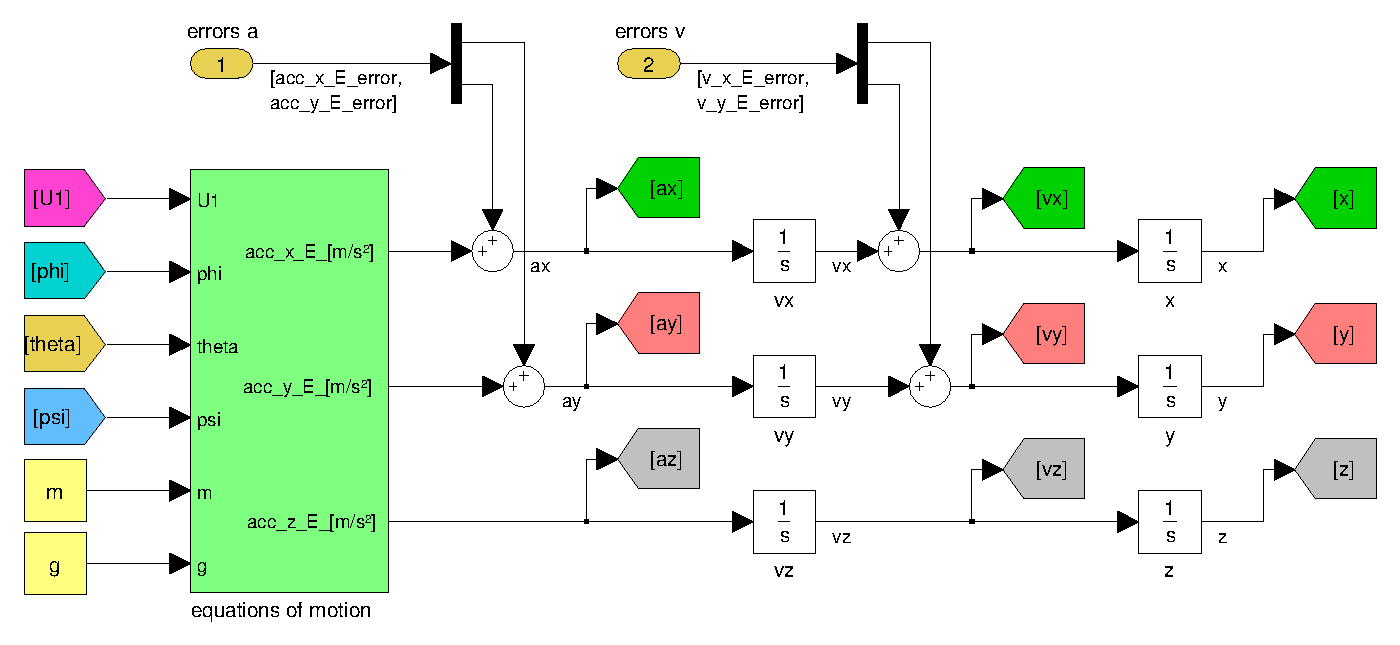
\includegraphics[width=1.0\textwidth]{03_Grafiken/MATLAB_Dynamics3.pdf}
	\caption{Blue section}
	\label{fig:MATLAB Dynamics3}
\end{figure}
At the 'input' of this section is one big, non-linear block, 'equations of motion'. It uses the 'output' of the red section, \textit{phi}, \textit{theta} and \textit{psi}, the sum of all propeller forces \textit{U1} and two constants m (mass of the quadrocopter) and g (gravitational acceleration) to calculate the accelerations in direction of x, y and z of the earthframe. These values get integrated to gain the linar speeds and the position of the quadrocopter. By using the inputs 'error a' and 'error v', it is possible to simulate wind.
\clearpage %neue Seite erzwingen

\subsubsection{Combination of all signals (yellow section)}\label{chapter_YELLOW_SECTION}
The yellow section shows the output vector of the dynamics block, called \textit{pos\_vel\_acc} (positions-velocities-accelerations).
\begin{figure}[htbp]
	\begin{minipage}[t]{8cm}
		\vspace{0pt}
		\begin{singlespace}
			\medskip
			\medskip
			\medskip
			\begin{itemize}
			\item position \textit{x} of earthframe
			\item position \textit{y} of earthframe
			\item position \textit{z} of earthframe
			\item angle \textit{phi} of bodyframe
			\item angle \textit{theta} of bodyframe
			\item angle \textit{psi} of bodyframe
			\item linear speed in direction of \textit{x}
			\item linear speed in direction of \textit{y}
			\item linear speed in direction of \textit{z}
			\item angular speed in direction of \textit{phi}
			\item angular speed in direction of \textit{theta}
			\item angular speed in direction of \textit{psi}
			\item linear acceleration in dir. of \textit{x}
			\item linear acceleration in dir. of \textit{y}
			\item linear acceleration in dir. of \textit{z}
			\item angular acceleration in dir. of \textit{phi}
			\item angular acceleration in dir. of \textit{theta}
			\item angular acceleration in dir. of \textit{psi}
			\item sum of all propeller forces
			\end{itemize}
		\end{singlespace}
	\end{minipage}
	\hfill
	\begin{minipage}[t]{6.5cm}
		\vspace{0pt}
		\centering
		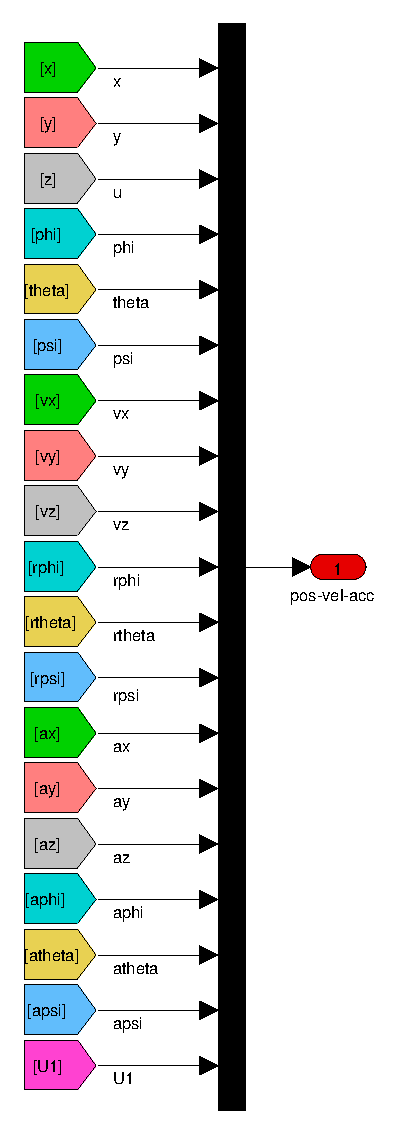
\includegraphics[width=6.15cm]{03_Grafiken/MATLAB_Dynamics4.pdf}
		\caption{Yellow Section}
		\label{fig:MATLAB Dynamics4}
	\end{minipage}
\end{figure}